% Copyright (c)  2019  FSC.
% Permission is granted to copy, distribute and/or modify this document
% under the terms of the GNU Free Documentation License, Version 1.3
% or any later version published by the Free Software Foundation;
% with no Invariant Sections, no Front-Cover Texts, and no Back-Cover Texts.
% A copy of the license is included in the section entitled "GNU
% Free Documentation License".

\chapter{Requisiti del sito}\label{chap:requisiti-del-sito}

\section{Requisiti di architettura}\label{sec:requisiti-di-architettura}

L'architettura informativa illustrata successivamente definisce una struttura 
generale dello \textit{schema gerarchico} indicante la logica di 
\textit{navigazione} suddividendo la web app in sezioni e sottosezioni. 

Per quanto riguarda l'area pubblica si prevede quanto segue:
\begin{itemize}
	\item \textbf{Landing page}
	\begin{itemize}
		\item \textbf{Funzionalità}
		\item \textbf{Su di noi}
	\end{itemize}
\item \textbf{Login}
\item \textbf{Registrazione}
\end{itemize}
Per quanto riguarda l'area privata, ovvero per ogni utente loggato si prevede 
quanto segue (\textit{con (*) viene indicata la molteplice quantità 
dell'oggetto a 
cui è affiancato}): 
\begin{itemize}
	\item \textbf{Home}
	\begin{itemize}
		\item \textbf{Progetti (*)} 
		\begin{itemize}
			\item \textbf{Sottoprogetti (*)}
			\begin{itemize}
				\item \textbf{Video (*)}
			\end{itemize}
		\item \textbf{Video (*)}
		\end{itemize}
	\end{itemize}
\end{itemize}
Indicativamente, la struttura di navigazione delle pagine più importante è 
definita mediante le seguenti \textit{gabbie logiche grafiche minimali}. Si 
riserverà al web designer il compito di definire meccanismi di navigazione e 
layout grafici più avanzati che ne determineranno il risultato finale.

% Copyright (c)  2019  FSC.
% Permission is granted to copy, distribute and/or modify this document
% under the terms of the GNU Free Documentation License, Version 1.3
% or any later version published by the Free Software Foundation;
% with no Invariant Sections, no Front-Cover Texts, and no Back-Cover Texts.
% A copy of the license is included in the section entitled "GNU
% Free Documentation License".

\begin{figure}[H]
	\centering
	\caption{Gabbia di occupazione di massima della landing page.}
	\label{fig:gabbie-massima:landing-page}
	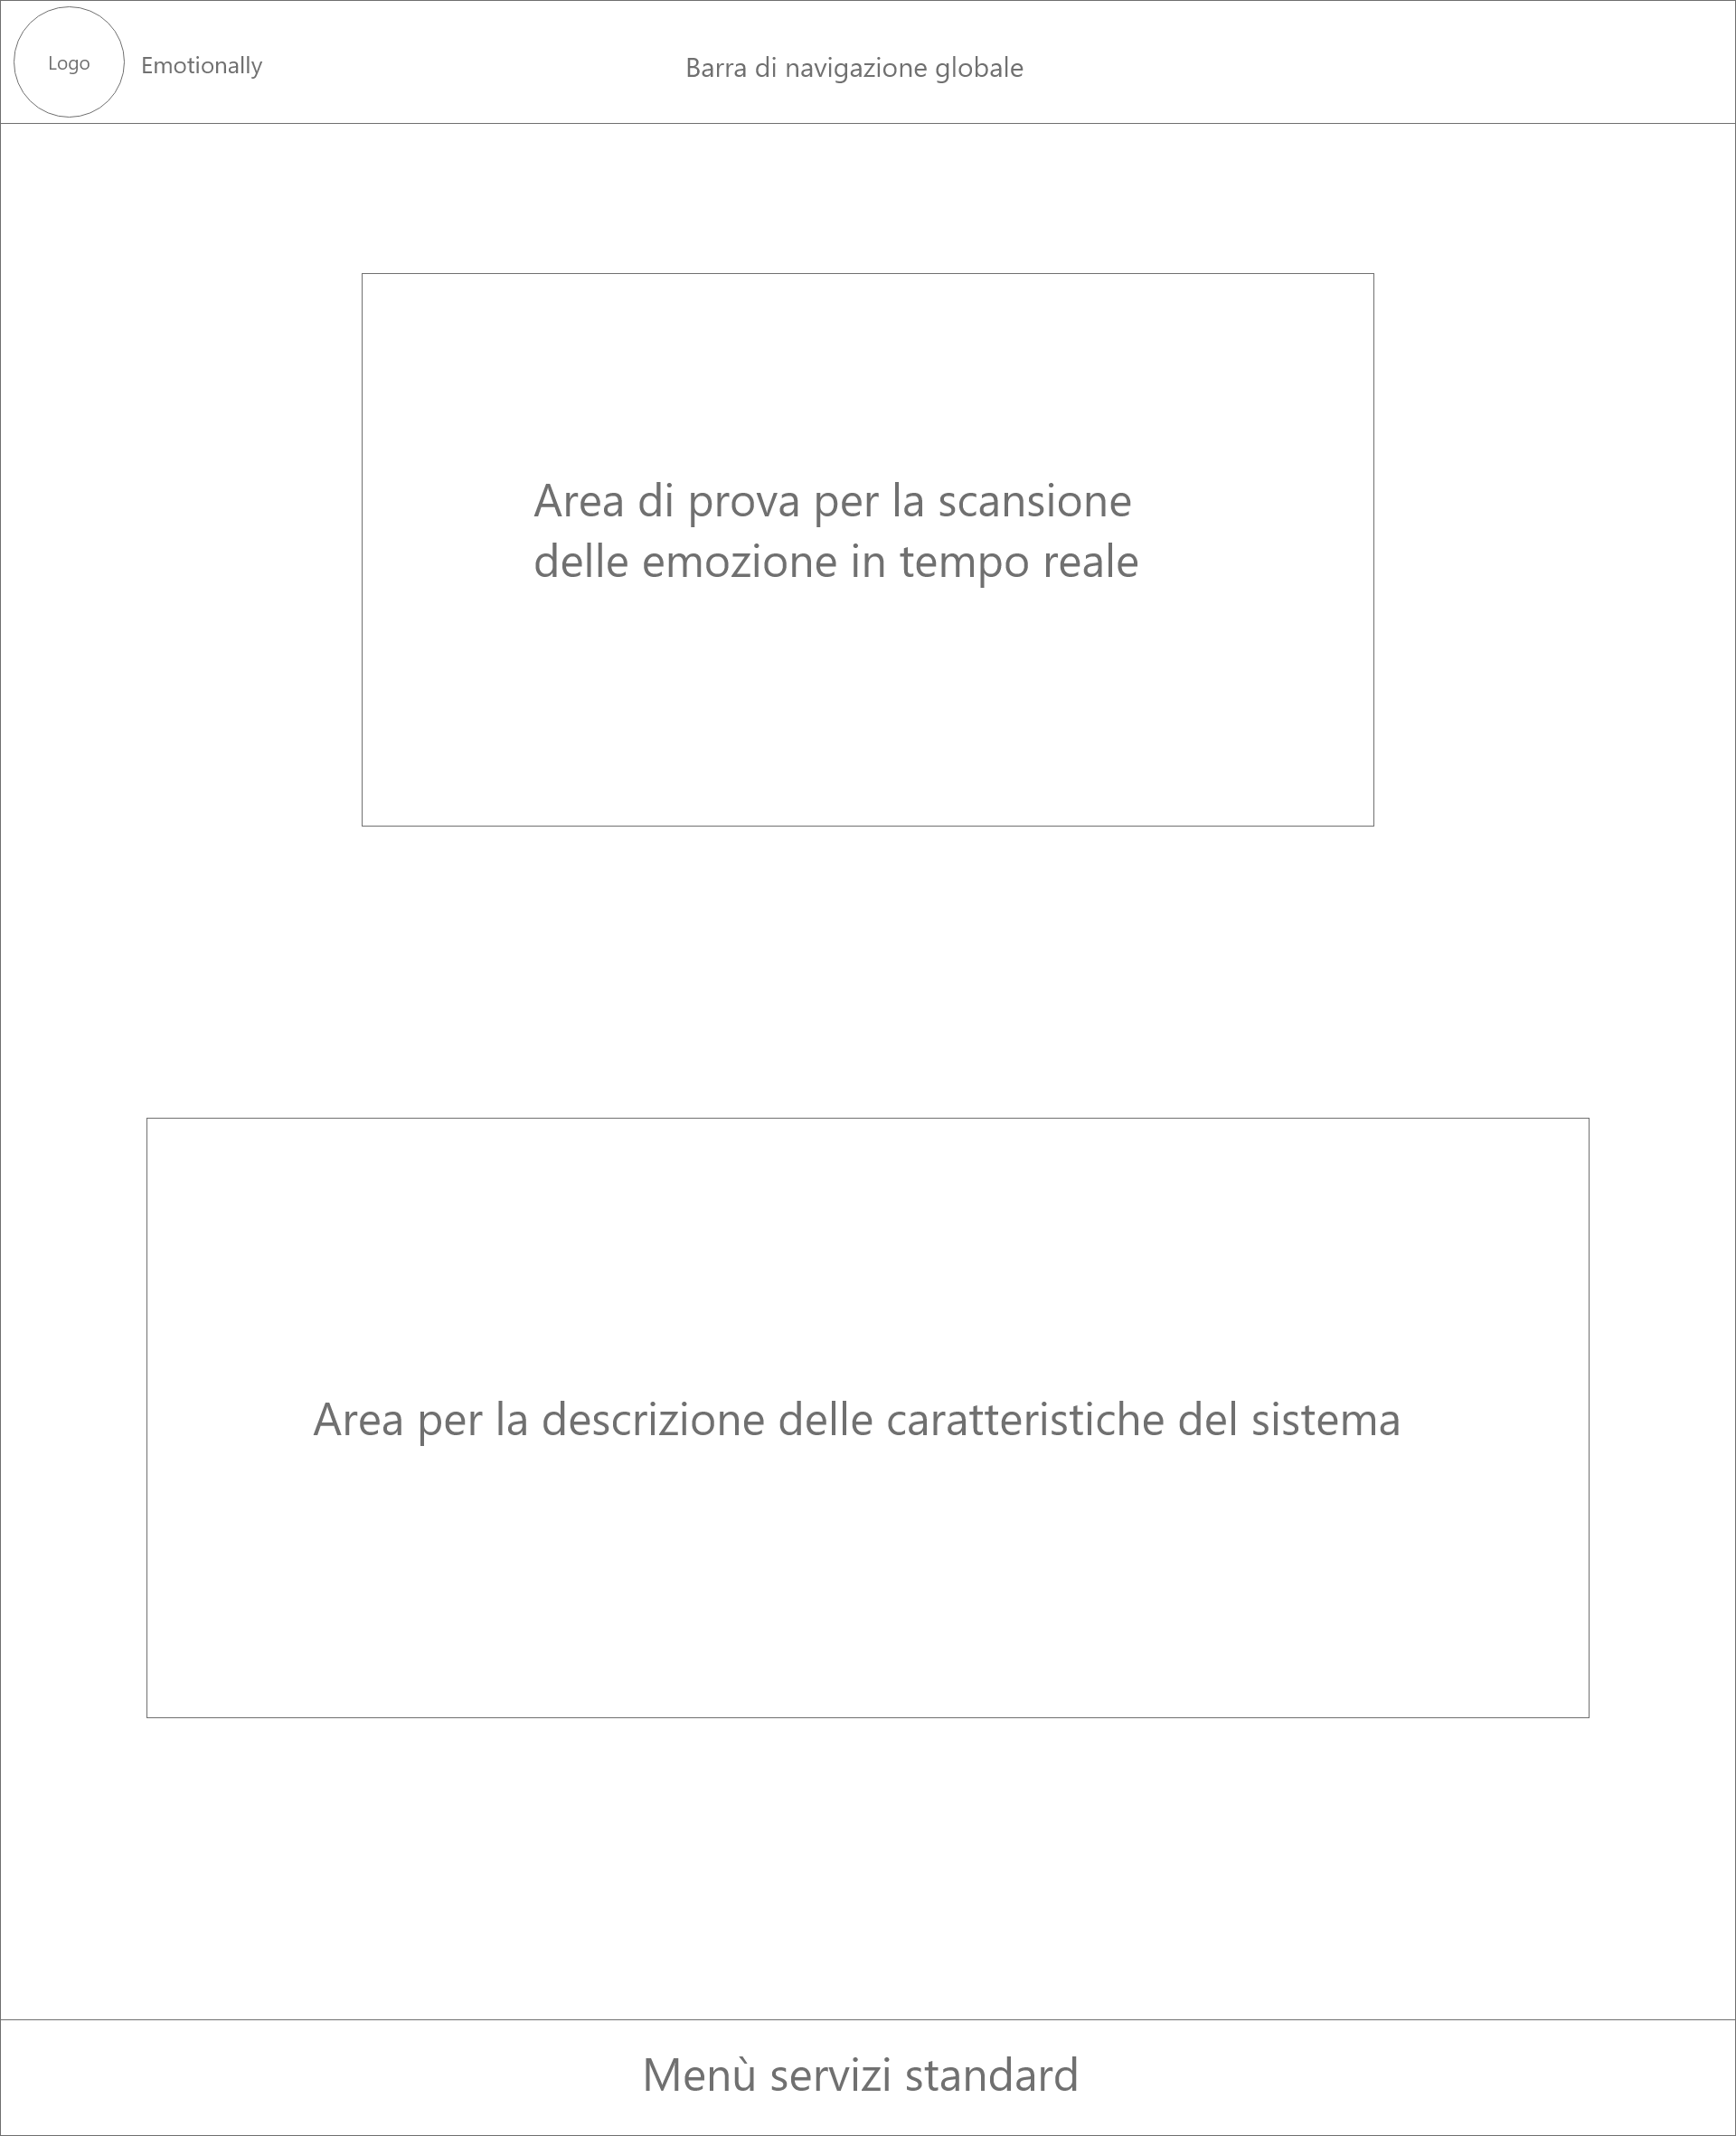
\includegraphics[width=\textwidth]{images/gabbie-di-massima/Landing}
\end{figure}

\begin{figure}[H]
	\centering
	\caption{Gabbia di occupazione di massima della pagina di login.}
	\label{fig:gabbie-massima:login}
	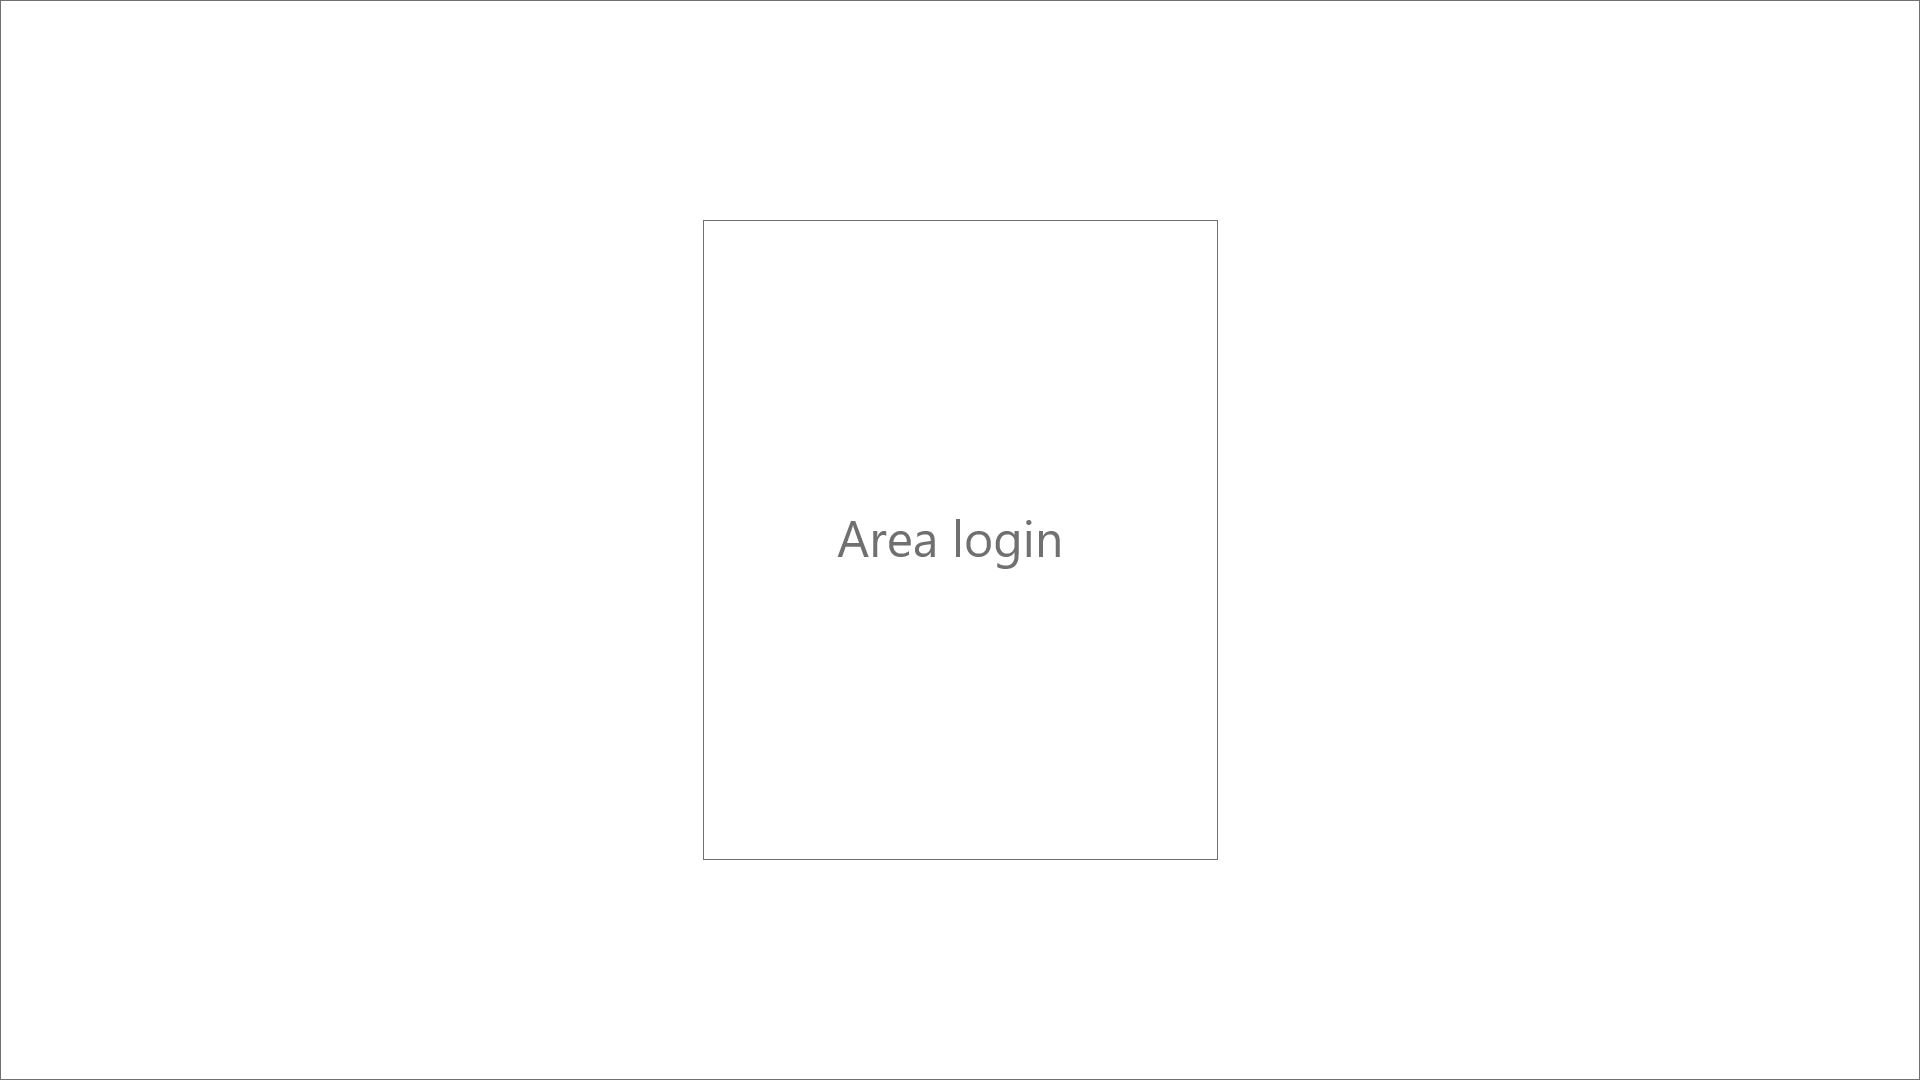
\includegraphics[width=\textwidth]{images/gabbie-di-massima/Login}
\end{figure}
\begin{figure}[H]
	\centering

	\caption{Gabbia di occupazione di massima della pagina di registrazione.}
	\label{fig:gabbie-massima:registrazione}
	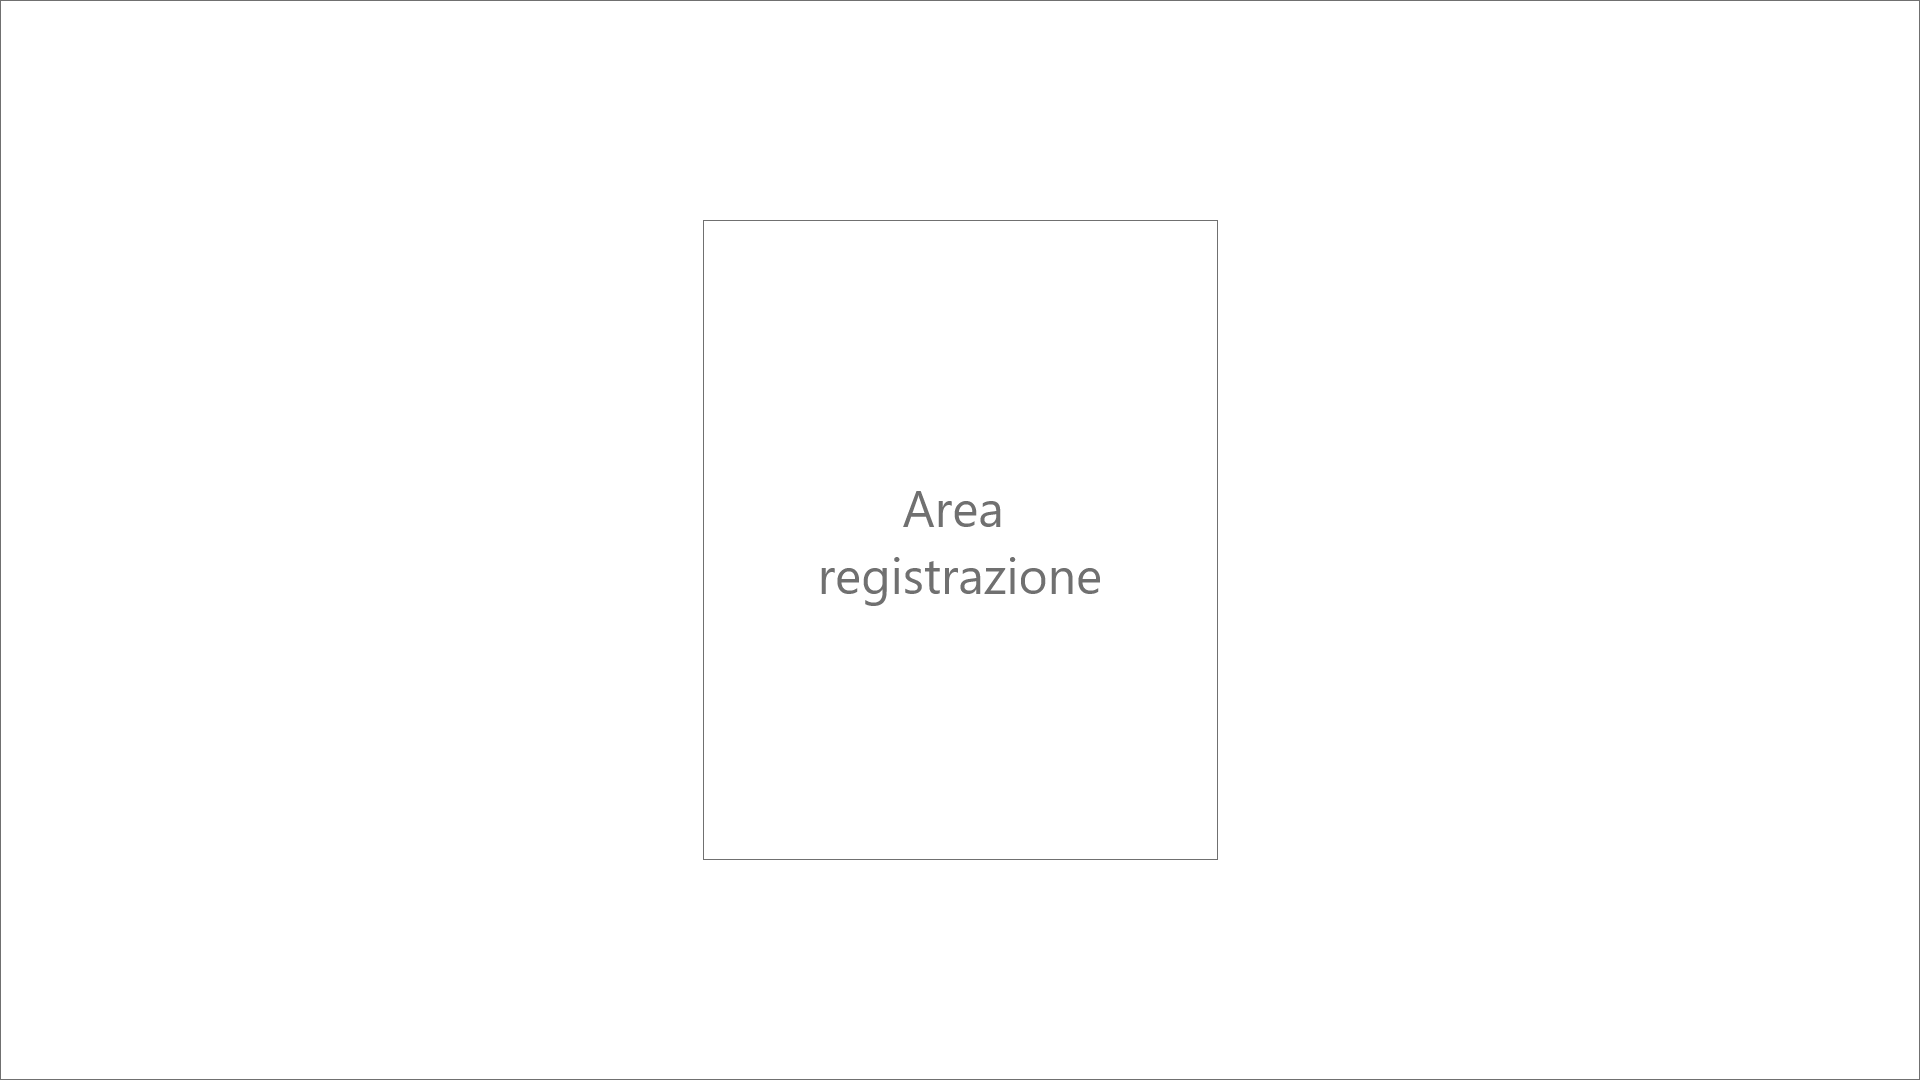
\includegraphics[width=\textwidth]{images/gabbie-di-massima/Registrazione}
\end{figure}

\begin{figure}[H]
	\centering
	\caption{Gabbia di occupazione di massima della home page.}
	\label{fig:gabbie-massima:home-page}
	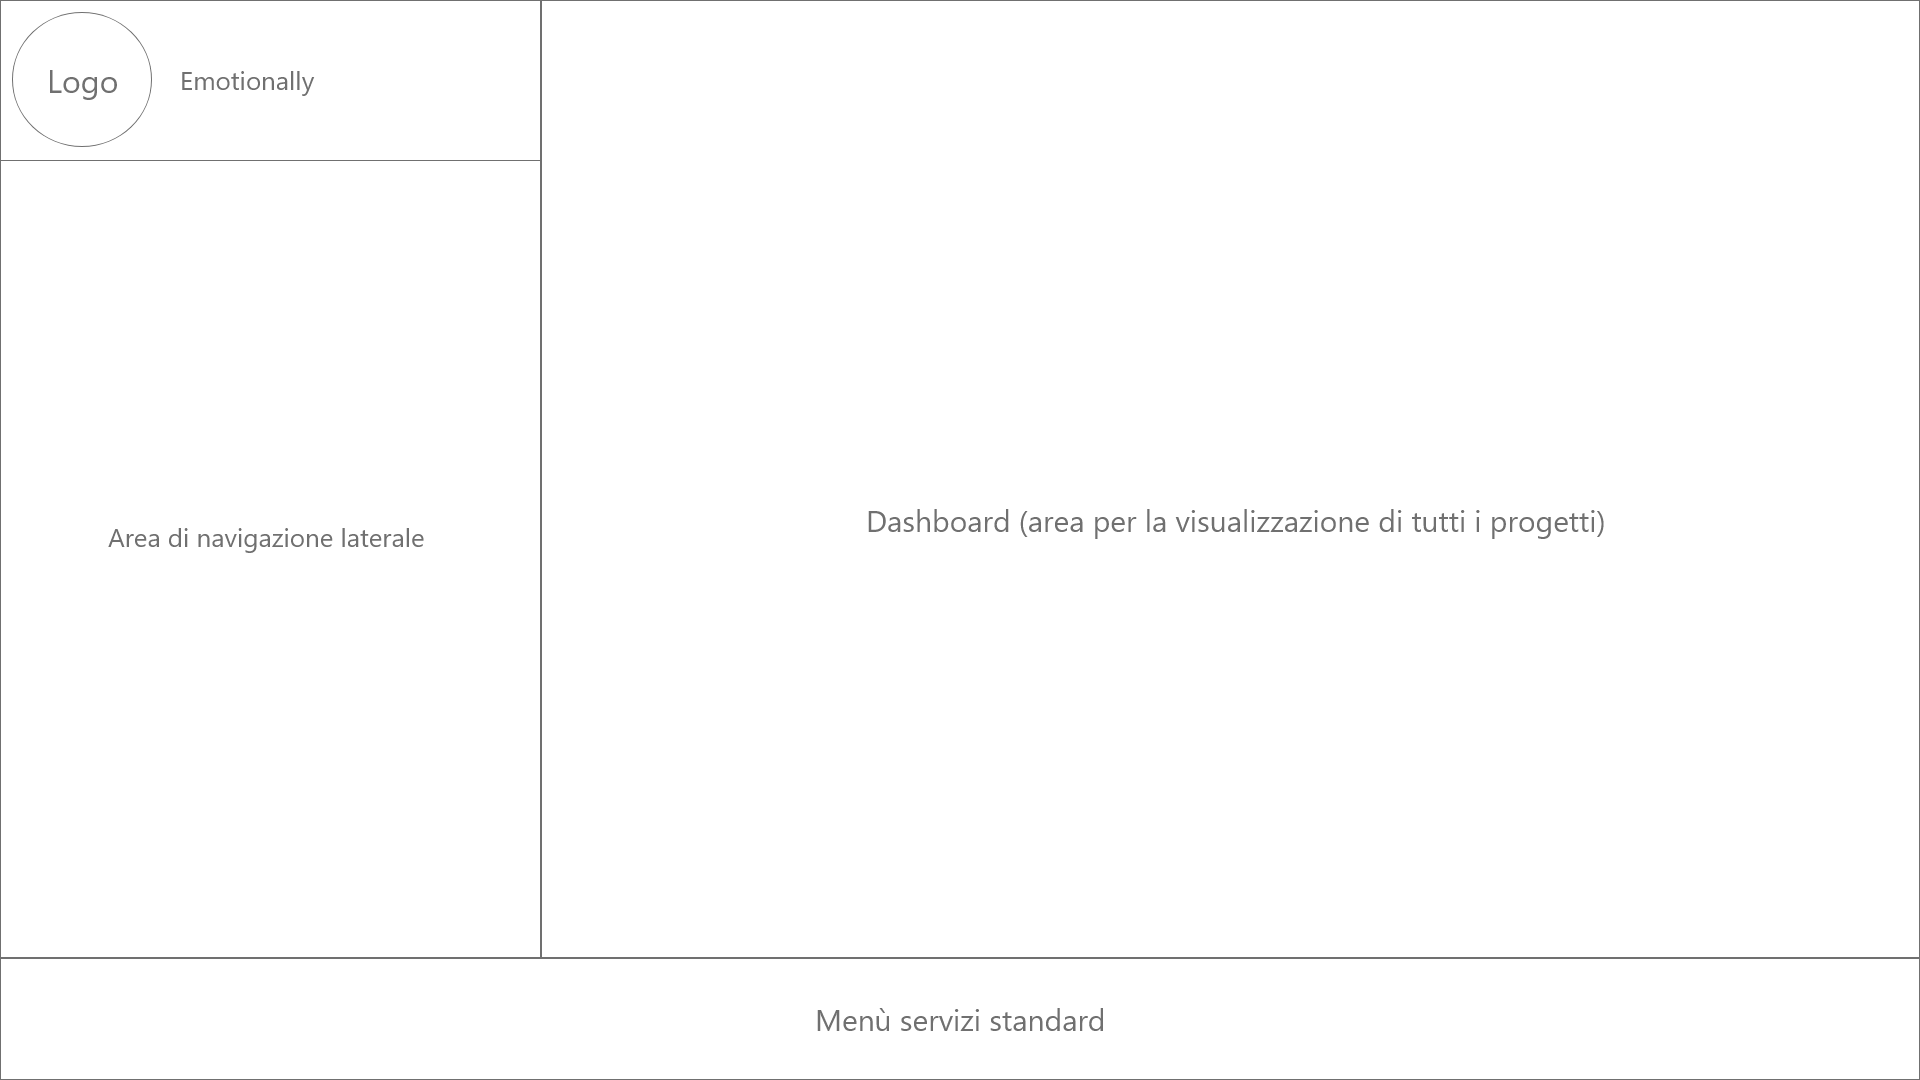
\includegraphics[width=\textwidth]{images/gabbie-di-massima/Home}
\end{figure}

\begin{figure}[H]
	\centering
	\caption{Gabbia di occupazione di massima della pagina di un progetto.}
	\label{fig:gabbie-massima:project}
	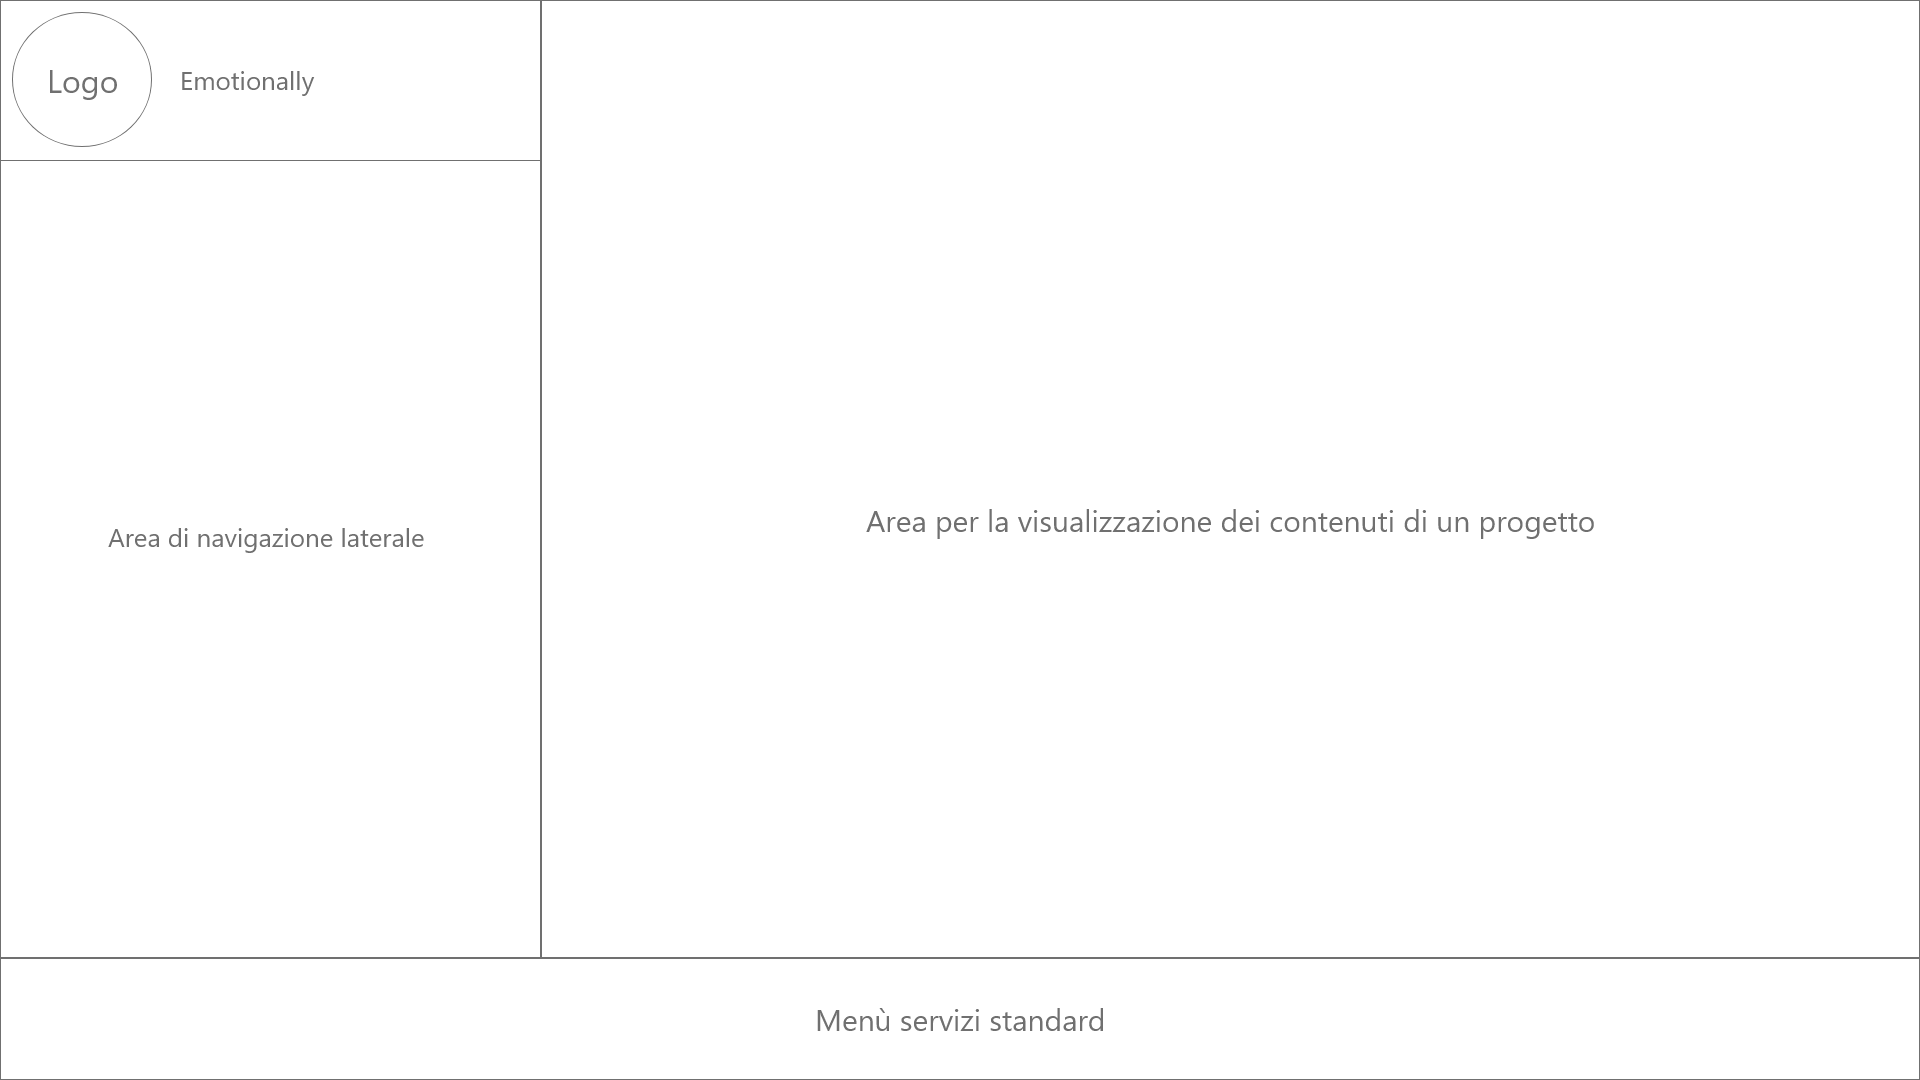
\includegraphics[width=\textwidth]{images/gabbie-di-massima/Progetto}
\end{figure}

\begin{figure}[H]
	\centering
	\caption{Gabbia di occupazione di massima della pagina di un video.}
	\label{fig:gabbie-massima:video}
	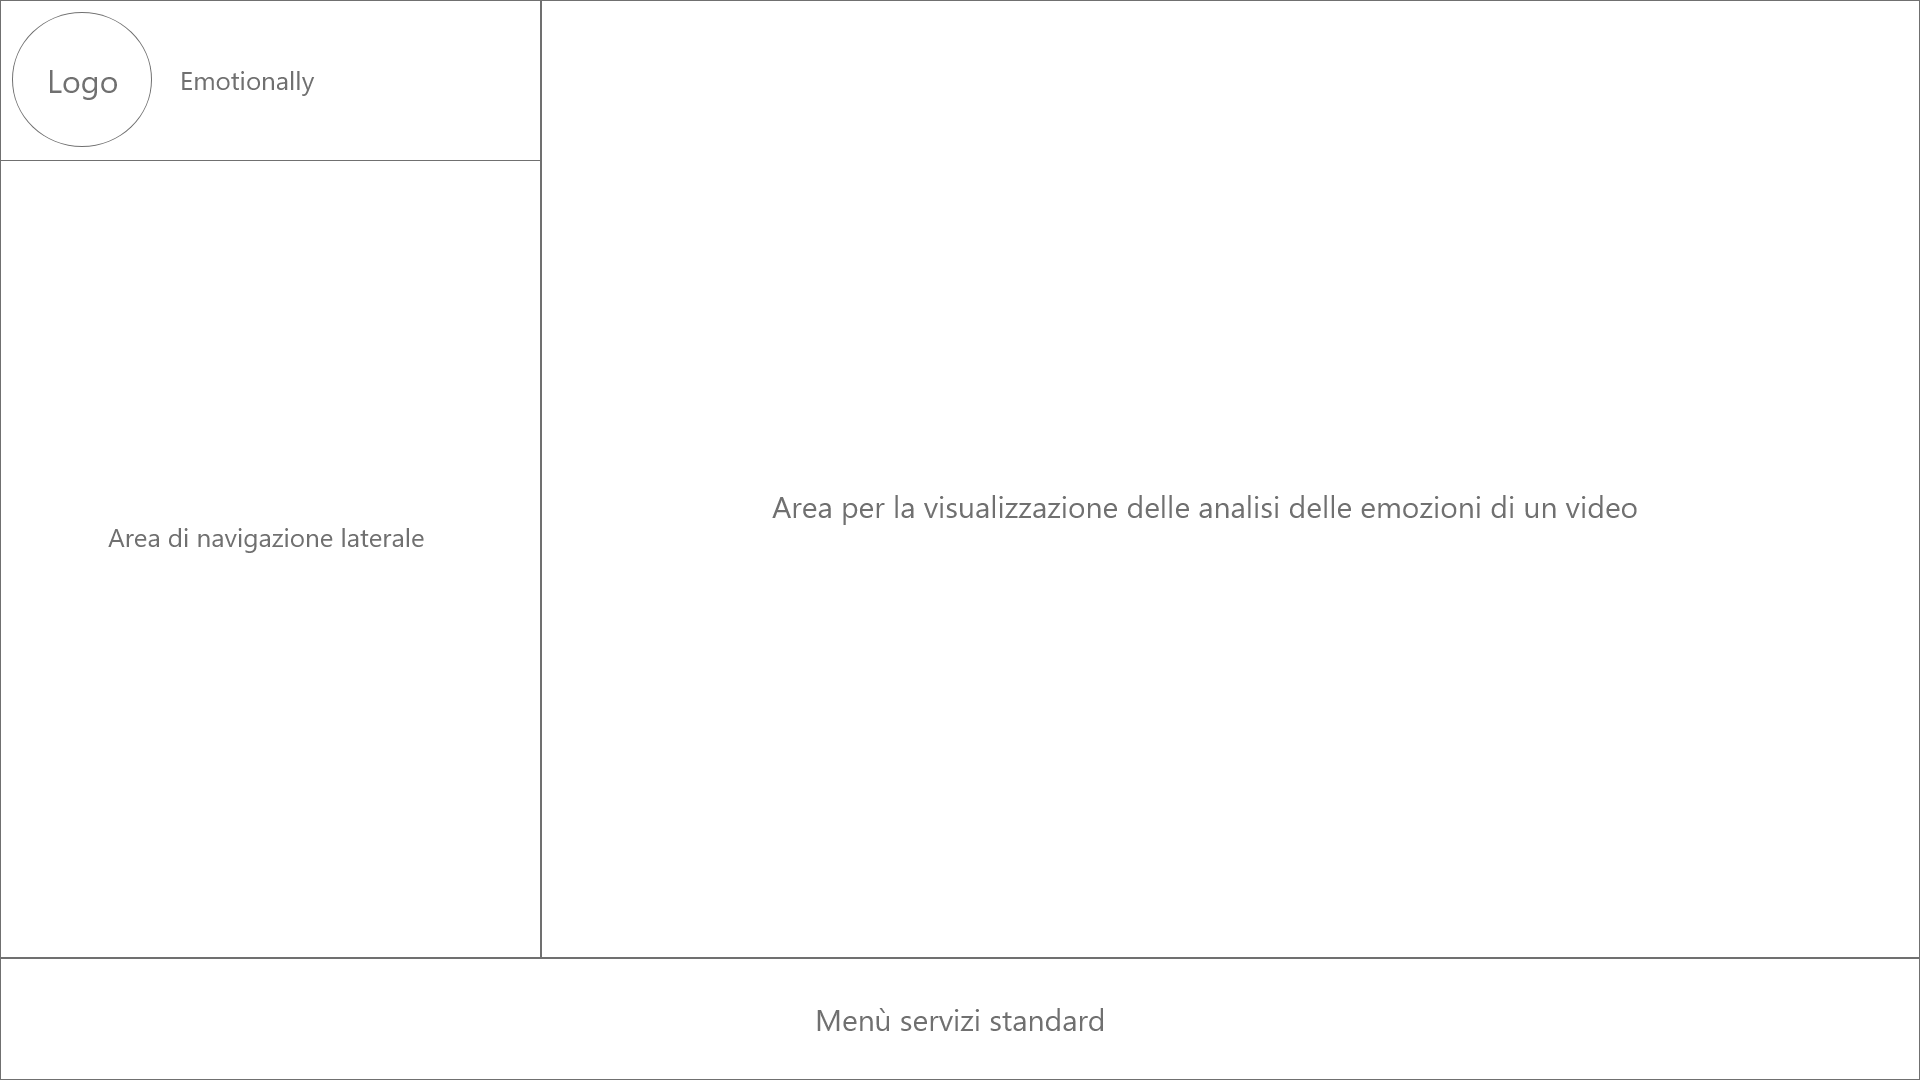
\includegraphics[width=\textwidth]{images/gabbie-di-massima/Video}
\end{figure}


\section{Requisiti di comunicazione}\label{sec:requisiti-di-comunicazione}
Le pagine interne della piattaforma web Emotionally dovranno essere 
graficamente coerenti tra di loro, fatta eccezione per la pagina di landing che 
dovrà presentare la piattaforma all'utente. La piattaforma web sarà bilingue 
(italiano e inglese).

Ogni pagina del sistema Emotionally dovrà:
\begin{itemize}
	\item contenere il logo del sistema stesso posizionato in alto a sinistra,
	\item avere un comportamento responsive: il sito deve ridimensionarsi 
	automaticamente al variare della risoluzionie video e della dimnesione 
	della finestra del browser,
	\item contenere caratteri la cui dimensione dovrà essere modificabile 
	dall'utente,
	\item avere una funzione accessibile, almeno di livello AA.
\end{itemize}
La landing page presenta, attraverso un'interfaccia chiara e usabile, le 
funzionalità del sistema e permette all'utente di approcciare il riconoscimento 
delle emozioni. 

Inoltre, per sottolineare la divisione tra il sistema e la landing page si è 
deciso di utilizzare un bottone di login differente rispetto allo stile dei 
link presenti nella navbar. A seguito del click del bottone, l'utente viene 
reindirizzato alla pagina di login che rappresenta, seppur in parte, lo stile 
grafico del sistema.

\section{Requisiti funzionali}\label{sec:requisiti-funzionali}

In questa sezione vengono illustrati i casi d'uso e le relative 
rappresentazioni tabellari riferiti alle diverse funzionalità che Emotionally 
offre ai suoi utenti. 

\subsection{Casi d'uso}

\begin{figure}[H]
	\centering
    \caption{I casi d'uso del sistema.}
    \label{fig:casi-duso}
    \resizebox{\textwidth}{!}{%
        % Copyright (c)  2019  FSC.
% Permission is granted to copy, distribute and/or modify this document
% under the terms of the GNU Free Documentation License, Version 1.3
% or any later version published by the Free Software Foundation;
% with no Invariant Sections, no Front-Cover Texts, and no Back-Cover Texts.
% A copy of the license is included in the section entitled "GNU
% Free Documentation License".

\begin{tikzpicture} 
    \begin{umlsystem}[x=6, y=20]{Emotionally} 
        % Define uses case of the GUEST
        \umlusecase[x=0,y=-2, name=Registration]{Registration} 
        \umlusecase[x=0,y=-3, name=TestAnalysis]{Test analysis}
        
        % Define uses case of the USER
        \umlusecase[x=0,y=-4, name=Login]{Login}
        \umlusecase[x=0,y=-5, name=Logout]{Logout}
        
        \umlusecase[x=0,y=-6, name=ProjectCreation]{Create project}
        \umlusecase[x=8, y=-2, name=ProjectEditing]{Edit project}
        \umlusecase[x=8, y=-3, name=ProjectRemoval]{Remove project}
        \umlusecase[x=0,y=-7, name=ProjectView]{View project}
        
        \umlusecase[x=8, y=-4, name=VideoUpload]{Upload video}
        \umlusecase[x=8, y=-5, name=VideoEditing]{Edit video}
        \umlusecase[x=8, y=-6, name=VideoRemoval]{Remove video}
        \umlusecase[x=8, y=-7, name=ViewVideo]{View video}
        
        \umlusecase[x=8, y=-8, name=SharingProject]{Share project}
        
        \umlusecase[y=-10, name=ReportView]{View report}
        \umlusecase[x=8, y=-9.5, name=VideoReportView]{View report of a video}
        \umlusecase[x=8, y=-10.5, name=ProjectReportView]{View report of a project}
        
        \umlusecase[x=8, y=-11.5, name=ReportDownload]{Download report}
        
        \umlusecase[y=-9, name=UserDataUpdate]{Update user data}
        \umlusecase[y=-8, name=DeleteAccount]{Delete account}
    \end{umlsystem} 
    
    % Define actor
    \umlactor[x=1, y=17.5]{Guest}
    \umlactor[x=1, y=14.5]{User}
    \umlactor[y=10.5]{Designer}
    \umlactor[x=2, y=10.5]{Analyst}
    
    % Define generalizzation between actor
    \umlinherit{User}{Guest}
    \umlinherit[geometry=|-|]{Designer}{User}
    \umlinherit[geometry=|-|]{Analyst}{User}
    
    % Define associations between actors and use cases
    \umlassoc{Guest}{Registration} 
    \umlassoc{Guest}{TestAnalysis} 
    \umlassoc{User}{Login} 
    \umlassoc{User}{Logout} 
    \umlassoc{User}{ProjectCreation}
    \umlassoc{User}{ProjectView}
    \umlassoc{User}{ReportView}
    \umlassoc{User}{UserDataUpdate}
    \umlassoc{User}{DeleteAccount}
    
    %Define extensions between use cases
    \umlHVHextend{ProjectEditing}{ProjectView}
    \umlHVHextend{ProjectRemoval}{ProjectView}
    \umlHVHextend{SharingProject}{ProjectView}
    \umlHVHextend{VideoUpload}{ProjectView}
    \umlHVHextend{VideoEditing}{ProjectView}
    \umlHVHextend{VideoRemoval}{ProjectView}
    \umlHVHextend{ViewVideo}{ProjectView}
    \umlHVextend{ReportDownload}{ReportView}
    
    % Define generalizzation between use cases
    \umlinherit[geometry=-|-]{VideoReportView}{ReportView}
    \umlinherit[geometry=-|-]{ProjectReportView}{ReportView}
\end{tikzpicture}

    }
\end{figure}

\subsection{Rappresentazione tabellare}
% TODO: Complete use case scenarios
\begin{table}[H]
	\centering
	\caption{Use Case: Registration}
	\label{tab:use-case-registration}
	\rowcolors{2}{gray!25}{white!0}
	\begin{longtable}{@{}|>{\centering\arraybackslash}m{.2\textwidth}|m{.7\textwidth}|@{}}
		\hline
		\rowcolor{emotionally-color!35}
		{\textbf{Nome caso d'uso}} & {\textbf{Registration (ID: 1)}} \\\hline
		\endfirsthead
		Descrizione & L'utente visitatore si registra alla piattaforma Emotionally.\\
		Attori & \begin{tabular}{m{0.9\linewidth}}~~\llap{\textbullet}~~Guest\\\end{tabular}\\
		Pre-condizioni & \begin{tabular}{m{0.9\linewidth}}~~\llap{\textbullet}~~L'utente non deve essere già registrato alla piattaforma\\\end{tabular}\\
		Sequenza delle azioni & \begin{tabular}{m{0.9\linewidth}}\hspace{0.0cm}1. Il guest chiede al sistema di potersi registrare alla piattaforma\\\hspace{0.0cm}2. Il sistema permette la registrazione chiedendo informazioni utili per la registrazione\\\hspace{0.5cm}\hspace{0.0cm}2.1. Fintantochè l'utente non inserisce una corretta email\\\hspace{0.5cm}\hspace{0.0cm}2.2. Il sistema chiede l'email\\\hspace{0.5cm}\hspace{0.0cm}2.3. L'utente inserisce l'email\\\hspace{0.0cm}3. Fintantochè l'utente non inserisce una password valida\\\hspace{0.5cm}\hspace{0.0cm}3.1. Il sistema chiede la password\\\hspace{0.5cm}\hspace{0.0cm}3.2. L'utente inserisce la password\\\hspace{0.0cm}4. Il sistema chiede il nome dell'utente\\\hspace{0.5cm}\hspace{0.0cm}4.1. L'utente inserisce il nome\\\hspace{0.0cm}5. Il sistema chiede il cognome dell'utente\\\hspace{0.5cm}\hspace{0.0cm}5.1. L'utente inserisce il cognome\\\hspace{0.0cm}6. Il sistema chiede il sesso dell'utente\\\hspace{0.5cm}\hspace{0.0cm}6.1. L'utente inserisce il sesso\\\end{tabular}\\
		Post-condizioni & \begin{tabular}{m{0.9\linewidth}}~~\llap{\textbullet}~~L'utente è registrato alla piattaforma\\\end{tabular}\\
		Scenario alternativo & \begin{tabular}{m{0.9\linewidth}}~~\llap{\textbullet}~~Uno scenario alternativo viene attivato al punto 2: il sistema informa l'utente che l'email inserita non è valida o corretta\\~~\llap{\textbullet}~~Uno scenario alternativo viene attivato al punto 3: il sistema informa l'utente che la password inserita non è valida\\\end{tabular}\\\hline
		
	\end{longtable}
\end{table}

\begin{table}[H]
	\centering
	\caption{Use Case: Test analysis}
	\label{tab:use-case-test-analysis}
	\rowcolors{2}{gray!25}{white!0}
	\begin{longtable}{@{}|>{\centering\arraybackslash}m{.2\textwidth}|m{.7\textwidth}|@{}}
		\hline
		\rowcolor{emotionally-color!35}
		{\textbf{Nome caso d'uso}} & {\textbf{Test analysis (ID: 2)}} \\\hline
		\endfirsthead
		Descrizione & L'utente visitatore vuole effettuare un test di prova di analisi delle emozioni\\
		Attori & \begin{tabular}{m{0.9\linewidth}}~~\llap{\textbullet}~~Guest\\~~\llap{\textbullet}~~User\\\end{tabular}\\
		Pre-condizioni & \begin{tabular}{m{0.9\linewidth}}~~\llap{\textbullet}~~L'utente non deve essere loggato alla piattaforma\\\end{tabular}\\
		Sequenza delle azioni & \begin{tabular}{m{0.9\linewidth}}\hspace{0.0cm}1. L'utente chiede al sistema di poter effettuare un'analisi di prova delle emozioni\\\hspace{0.0cm}2. Il sistema permette l'analisi di prova richiesta\\\end{tabular}\\
		Post-condizioni & \begin{tabular}{m{0.9\linewidth}}~~\llap{\textbullet}~~L'analisi di prova delle emozioni è stata effettuata.\\\end{tabular}\\
		Scenario alternativo & \begin{tabular}{m{0.9\linewidth}}~~\llap{\textbullet}~~Nessuno\\\end{tabular}\\\hline
		
	\end{longtable}
\end{table}

\begin{table}[H]
	\centering
	\caption{Use Case: Login}
	\label{tab:use-case-login}
	\rowcolors{2}{gray!25}{white!0}
	\begin{longtable}{@{}|>{\centering\arraybackslash}m{.2\textwidth}|m{.7\textwidth}|@{}}
		\hline
		\rowcolor{emotionally-color!35}
		{\textbf{Nome caso d'uso}} & {\textbf{Login (ID: 3)}} \\\hline
		\endfirsthead
		Descrizione & L'utente vuole effettuare l'accesso alla piattaforma Emotionally\\
		Attori & \begin{tabular}{m{0.9\linewidth}}~~\llap{\textbullet}~~User\\\end{tabular}\\
		Pre-condizioni & \begin{tabular}{m{0.9\linewidth}}~~\llap{\textbullet}~~L'utente deve aver già effettuato la registrazione\\\end{tabular}\\
		Sequenza delle azioni & \begin{tabular}{m{0.9\linewidth}}\hspace{0.0cm}1. L'utente chiede al sistema di poter effettuare il login\\\hspace{0.0cm}2. Il sistema chiede all'utente di inserire le informazioni necessarie per effettuare l'accesso\\\hspace{0.0cm}3. Fintantochè l'utente non inserisce un'email valida\\\hspace{0.5cm}\hspace{0.0cm}3.1. Il sistema chiede all'utente di inserire l'email\\\hspace{0.5cm}\hspace{0.0cm}3.2. L'utente inserisce l'email\\\hspace{0.0cm}4. Fintantochè l'utente non inserisce una password valida\\\hspace{0.5cm}\hspace{0.0cm}4.1. Il sistema chiede all'utente di inserire la password\\\hspace{0.5cm}\hspace{0.0cm}4.2. L'utente inserisce la password\\\hspace{0.0cm}5. Il sistema fa accedere l'utente alla piattaforma\\\end{tabular}\\
		Post-condizioni & \begin{tabular}{m{0.9\linewidth}}~~\llap{\textbullet}~~L'utente ha effettuato il login\\\end{tabular}\\
		Scenario alternativo & \begin{tabular}{m{0.9\linewidth}}~~\llap{\textbullet}~~Uno scenario alternativo viene innescato al punto 3: il sistema avvisa l'utente che l'email inserita non è valida.\\~~\llap{\textbullet}~~Uno scenario alternativo viene innescato al punto 4: il sistema avvisa l'utente che la password inserita non è valida.\\\end{tabular}\\\hline
		
	\end{longtable}
\end{table}

\begin{table}[H]
	\centering
	\caption{Use Case: Logout}
	\label{tab:use-case-logout}
	\rowcolors{2}{gray!25}{white!0}
	\begin{longtable}{@{}|>{\centering\arraybackslash}m{.2\textwidth}|m{.7\textwidth}|@{}}
		\hline
		\rowcolor{emotionally-color!35}
		{\textbf{Nome caso d'uso}} & {\textbf{Logout (ID: 4)}} \\\hline
		\endfirsthead
		Descrizione & L'utente vuole uscire dalla piattaforma Emotionally.\\
		Attori & \begin{tabular}{m{0.9\linewidth}}~~\llap{\textbullet}~~User\\\end{tabular}\\
		Pre-condizioni & \begin{tabular}{m{0.9\linewidth}}~~\llap{\textbullet}~~L'utente deve essere già loggato alla piattaforma\\\end{tabular}\\
		Sequenza delle azioni & \begin{tabular}{m{0.9\linewidth}}\hspace{0.0cm}1. L'utente chiede al sistema di porter effettuare il logout\\\hspace{0.0cm}2. Il sistema chiede all'utente la conferma di logout\\\hspace{0.0cm}3. Se l'utente conferma\\\hspace{0.5cm}\hspace{0.0cm}3.1. Il sistema permetterà l'uscita dalla piattaforma\\\hspace{0.0cm}4. Altrimenti\\\hspace{0.5cm}\hspace{0.0cm}4.1. Il sistema fermerà il processo di logout\\\end{tabular}\\
		Post-condizioni & \begin{tabular}{m{0.9\linewidth}}~~\llap{\textbullet}~~L'utente ha effettuato il logout\\\end{tabular}\\
		Scenario alternativo & \begin{tabular}{m{0.9\linewidth}}~~\llap{\textbullet}~~Nessuno\\\end{tabular}\\\hline
		
	\end{longtable}
\end{table}

\begin{table}[H]
	\centering
	\caption{Use Case: Create project}
	\label{tab:use-case-create-project}
	\rowcolors{2}{gray!25}{white!0}
	\begin{longtable}{@{}|>{\centering\arraybackslash}m{.2\textwidth}|m{.7\textwidth}|@{}}
		\hline
		\rowcolor{emotionally-color!35}
		{\textbf{Nome caso d'uso}} & {\textbf{Create project (ID: 5)}} \\\hline
		\endfirsthead
		Descrizione & L'utente vuole creare un nuovo progetto.\\
		Attori & \begin{tabular}{m{0.9\linewidth}}~~\llap{\textbullet}~~User\\\end{tabular}\\
		Pre-condizioni & \begin{tabular}{m{0.9\linewidth}}~~\llap{\textbullet}~~L'utente deve essere loggato alla piattaforma\\\end{tabular}\\
		Sequenza delle azioni & \begin{tabular}{m{0.9\linewidth}}\hspace{0.0cm}1. L'utente chiede al sistema di poter creare un nuovo progetto\\\hspace{0.0cm}2. Il sistema chiede delle informazioni relative al nuovo progetto\\\hspace{0.0cm}3. Fintantochè l'utente non inserisce un nome di progetto valido\\\hspace{0.5cm}\hspace{0.0cm}3.1. Il sistema chiede all'utente di inserire il nome di progetto\\\hspace{0.5cm}\hspace{0.0cm}3.2. L'utente inserisce il nome di progetto\\\hspace{0.0cm}4. Fintantochè l'utente non inserisce una cartella padre valido\\\hspace{0.5cm}\hspace{0.0cm}4.1. Il sistema chiede all'utente di inserire la cartella padre del progetto\\\hspace{0.5cm}\hspace{0.0cm}4.2. L'utente inserisce la cartella padre del progetto\\\hspace{0.0cm}5. Il sistema effettua la creazione del nuovo progetto\\\end{tabular}\\
		Post-condizioni & \begin{tabular}{m{0.9\linewidth}}~~\llap{\textbullet}~~L'utente ha creato un nuovo progetto\\\end{tabular}\\
		Scenario alternativo & \begin{tabular}{m{0.9\linewidth}}~~\llap{\textbullet}~~Uno scenario alternativo viene innescato al punto 3: il sistema avvisa l'utente di aver inserito un nome di progetto non valido.\\~~\llap{\textbullet}~~Uno scenario alternativo viene innescato al punto 4: Il sistema avvisa l'utente di aver inserito una cartella padre errate\\\end{tabular}\\\hline
		
	\end{longtable}
\end{table}

\begin{table}[H]
	\centering
	\caption{Use Case: View project}
	\label{tab:use-case-view-project}
	\rowcolors{2}{gray!25}{white!0}
	\begin{longtable}{@{}|>{\centering\arraybackslash}m{.2\textwidth}|m{.7\textwidth}|@{}}
		\hline
		\rowcolor{emotionally-color!35}
		{\textbf{Nome caso d'uso}} & {\textbf{View project (ID: 6)}} \\\hline
		\endfirsthead
		Descrizione & L'utente vuole visualizzare uno dei suoi progetti.\\
		Attori & \begin{tabular}{m{0.9\linewidth}}~~\llap{\textbullet}~~User\\\end{tabular}\\
		Pre-condizioni & \begin{tabular}{m{0.9\linewidth}}~~\llap{\textbullet}~~L'utente deve aver effettuato la procedura di login\\~~\llap{\textbullet}~~L'utente deve aver già creato il progetto che vuole visualizzare\\\end{tabular}\\
		Sequenza delle azioni & \begin{tabular}{m{0.9\linewidth}}\hspace{0.0cm}1. L'utente chiede al sistema di poter visualizzare un suo progetto\\\hspace{0.0cm}2. Il sistema permette la visualizzazione del progetto scelto all'utente richiedente\\\end{tabular}\\
		Post-condizioni & \begin{tabular}{m{0.9\linewidth}}~~\llap{\textbullet}~~L'utente visualizza il progetto\\\end{tabular}\\
		Scenario alternativo & \begin{tabular}{m{0.9\linewidth}}~~\llap{\textbullet}~~Nessuno\\\end{tabular}\\\hline
		
	\end{longtable}
\end{table}

\begin{table}[H]
	\centering
	\caption{Use Case: Edit project}
	\label{tab:use-case-edit-project}
	\rowcolors{2}{gray!25}{white!0}
	\begin{longtable}{@{}|>{\centering\arraybackslash}m{.2\textwidth}|m{.7\textwidth}|@{}}
		\hline
		\rowcolor{emotionally-color!35}
		{\textbf{Nome caso d'uso}} & {\textbf{Edit project (ID: 7)}} \\\hline
		\endfirsthead
		Descrizione & L'utente vuole modificare un progetto da lui scelto.\\
		Attori & \begin{tabular}{m{0.9\linewidth}}~~\llap{\textbullet}~~User\\\end{tabular}\\
		Pre-condizioni & \begin{tabular}{m{0.9\linewidth}}~~\llap{\textbullet}~~L'utente deve essere loggato alla piattaforma\\~~\llap{\textbullet}~~Il progetto scelto dall'utente deve essere già stato creato\\\end{tabular}\\
		Sequenza delle azioni & \begin{tabular}{m{0.9\linewidth}}\hspace{0.0cm}1. L'utente chiede al sistema di porter modificare il progetto\\\hspace{0.0cm}2. Il sistema permette all'utente di modificare il progetto richiesto\\\hspace{0.0cm}3. Se l'utente chiede di rinominare il progetto\\\hspace{0.5cm}\hspace{0.0cm}3.1. Fintantochè il nuovo nome del progetto non è valido\\\hspace{1.0cm}\hspace{0.5cm}\hspace{0.0cm}3.1.1. Il sistema chiede all'utente di inserire il nuovo nome del progetto\\\hspace{1.0cm}\hspace{0.5cm}\hspace{0.0cm}3.1.2. L'utente inserisce il nuovo nome del progetto\\\hspace{0.0cm}4. Se l'utente chiede di spostare un video\\\hspace{0.5cm}\hspace{0.0cm}4.1. Il sistema chiede all'utente in quale progetto vuole spostarlo\\\hspace{0.5cm}\hspace{0.0cm}4.2. Se il video è già presente nel progetto in cui si intende spostarlo\\\hspace{1.0cm}\hspace{0.5cm}\hspace{0.0cm}4.2.1. Il sistema chiede all'utente conferma per lo spostamento del video\\\hspace{0.5cm}\hspace{0.0cm}4.3. Altrimenti\\\end{tabular}\\
		Post-condizioni & \begin{tabular}{m{0.9\linewidth}}~~\llap{\textbullet}~~Il progetto scelto è stato modificato\\\end{tabular}\\
		Scenario alternativo & \begin{tabular}{m{0.9\linewidth}}~~\llap{\textbullet}~~Uno scenario alternativo viene innescato al punto 4.2: Il sistema chiede all'utente se vuole rinominare il video, se vuole sovrascrivere il video con lo stesso nome di quello che si vuole spostare o se si vuole annullare l'operazione\\\end{tabular}\\\hline
		
	\end{longtable}
\end{table}

\begin{table}[H]
	\centering
	\caption{Use Case: Remove project}
	\label{tab:use-case-remove-project}
	\rowcolors{2}{gray!25}{white!0}
	\begin{longtable}{@{}|>{\centering\arraybackslash}m{.2\textwidth}|m{.7\textwidth}|@{}}
		\hline
		\rowcolor{emotionally-color!35}
		{\textbf{Nome caso d'uso}} & {\textbf{Remove project (ID: 8)}} \\\hline
		\endfirsthead
		Descrizione & L'utente vuole rimuovere un suo progetto dalla piattaforma.\\
		Attori & \begin{tabular}{m{0.9\linewidth}}~~\llap{\textbullet}~~User\\\end{tabular}\\
		Pre-condizioni & \begin{tabular}{m{0.9\linewidth}}~~\llap{\textbullet}~~L'utente deve aver effettuato la procedura di login\\~~\llap{\textbullet}~~Il progetto da eliminare deve essere stato già creato dall'utente\\\end{tabular}\\
		Sequenza delle azioni & \begin{tabular}{m{0.9\linewidth}}\hspace{0.0cm}1. L'utente chiede al sistema di poter rimuovere il progetto scelto\\\hspace{0.0cm}2. Il sistema chiede all'utente conferma dell'eliminazione del progetto scelto\\\hspace{0.0cm}3. Se l'utente confema\\\hspace{0.5cm}\hspace{0.0cm}3.1. Il sistema provvede all'eliminazione del progetto scelto\\\hspace{0.0cm}4. Altrimenti\\\hspace{0.5cm}\hspace{0.0cm}4.1. Il sistema annullerà l'operazione\\\end{tabular}\\
		Post-condizioni & \begin{tabular}{m{0.9\linewidth}}~~\llap{\textbullet}~~Il progetto scelto dall'utente è stato eliminato\\\end{tabular}\\
		Scenario alternativo & \begin{tabular}{m{0.9\linewidth}}~~\llap{\textbullet}~~Nessuno\\\end{tabular}\\\hline
		
	\end{longtable}
\end{table}

\begin{table}[H]
	\centering
	\caption{Use Case: Upload video}
	\label{tab:use-case-upload-video}
	\rowcolors{2}{gray!25}{white!0}
	\begin{longtable}{@{}|>{\centering\arraybackslash}m{.2\textwidth}|m{.7\textwidth}|@{}}
		\hline
		\rowcolor{emotionally-color!35}
		{\textbf{Nome caso d'uso}} & {\textbf{Upload video (ID: 9)}} \\\hline
		\endfirsthead
		Descrizione & L'utente vuole inserire un nuovo video.\\
		Attori & \begin{tabular}{m{0.9\linewidth}}~~\llap{\textbullet}~~User\\\end{tabular}\\
		Pre-condizioni & \begin{tabular}{m{0.9\linewidth}}~~\llap{\textbullet}~~L'utente deve essere loggato nel sistema\\~~\llap{\textbullet}~~Il progetto in cui inserire il video deve essere stato già creato\\~~\llap{\textbullet}~~Il video non deve essere stato già inserito nel progetto in cui lo vuole caricare\\\end{tabular}\\
		Sequenza delle azioni & \begin{tabular}{m{0.9\linewidth}}\hspace{0.0cm}1. L'utente richiede al sistema di poter inserire un nuovo video\\\hspace{0.0cm}2. Finantochè l'utente non confermi o non annulli l'operazione\\\hspace{0.5cm}\hspace{0.0cm}2.1. Il sistema chiede all'utente di inserire il video\\\hspace{0.5cm}\hspace{0.0cm}2.2. L'utente inserisce il video che vuole caricare\\\hspace{0.5cm}\hspace{0.0cm}2.3. Se l'utente vuole modificare il nome del video da caricare\\\hspace{1.0cm}\hspace{0.5cm}\hspace{0.0cm}2.3.1. Il sistema permette all'utente di modificare il nome del video\\\hspace{1.0cm}\hspace{0.5cm}\hspace{0.0cm}2.3.2. L'utente inserisce il nome del video\\\hspace{0.5cm}\hspace{0.0cm}2.4. Altrimenti\\\hspace{1.0cm}\hspace{0.5cm}\hspace{0.0cm}2.4.1. Il sistema lascerà il nome del video al suo stesso inserimento\\\end{tabular}\\
		Post-condizioni & \begin{tabular}{m{0.9\linewidth}}~~\llap{\textbullet}~~L'utente ha inserito un nuovo video\\\end{tabular}\\
		Scenario alternativo & \begin{tabular}{m{0.9\linewidth}}~~\llap{\textbullet}~~Nessuno\\\end{tabular}\\\hline
		
	\end{longtable}
\end{table}

\begin{table}[H]
	\centering
	\caption{Use Case: Edit video}
	\label{tab:use-case-edit-video}
	\rowcolors{2}{gray!25}{white!0}
	\begin{longtable}{@{}|>{\centering\arraybackslash}m{.2\textwidth}|m{.7\textwidth}|@{}}
		\hline
		\rowcolor{emotionally-color!35}
		{\textbf{Nome caso d'uso}} & {\textbf{Edit video (ID: 10)}} \\\hline
		\endfirsthead
		Descrizione & L'utente vuole modificare un video da lui scelto.\\
		Attori & \begin{tabular}{m{0.9\linewidth}}~~\llap{\textbullet}~~User\\\end{tabular}\\
		Pre-condizioni & \begin{tabular}{m{0.9\linewidth}}~~\llap{\textbullet}~~L'utente deve aver effettuato la procedura di login\\~~\llap{\textbullet}~~Il video deve essere stato già caricato\\\end{tabular}\\
		Sequenza delle azioni & \begin{tabular}{m{0.9\linewidth}}\hspace{0.0cm}1. L'utente chiede al sistema di poter effettuare modifiche al video selezionato\\\hspace{0.0cm}2. Il sistema permette all'utente di modificare le informazioni inerenti al video\\\hspace{0.0cm}3. Fintantochè l'utente non salvi le modifiche o annulli l'operazione\\\hspace{0.5cm}\hspace{0.0cm}3.1. Se l'utente vuole modificare il nome del video selezionato\\\hspace{1.0cm}\hspace{0.5cm}\hspace{0.0cm}3.1.1. Fintantochè l'utente non inserisce un nome del video valido\\\hspace{1.5cm}\hspace{1.0cm}\hspace{0.5cm}\hspace{0.0cm}3.1.1.1. Il sistema chiede all'utente il nuovo nome del video\\\hspace{1.5cm}\hspace{1.0cm}\hspace{0.5cm}\hspace{0.0cm}3.1.1.2. L'utente inserisce il nome del video\\\hspace{0.5cm}\hspace{0.0cm}3.2. Se l'utente vuole modificare l'intervallo di analisi del video\\\hspace{1.0cm}\hspace{0.5cm}\hspace{0.0cm}3.2.1. Il sistema chiede all'utente di selezionare un intervallo di analisi\\\hspace{1.0cm}\hspace{0.5cm}\hspace{0.0cm}3.2.2. L'utente inserisce l'intervallo di analisi del video richiesto\\\end{tabular}\\
		Post-condizioni & \begin{tabular}{m{0.9\linewidth}}~~\llap{\textbullet}~~L'utente ha modificato il video selezionato\\\end{tabular}\\
		Scenario alternativo & \begin{tabular}{m{0.9\linewidth}}~~\llap{\textbullet}~~Uno scenario alternativo si innesca nel punto 3.1.1: il sistema avverte l'utente che il nome inserito non è valido\\\end{tabular}\\\hline
		
	\end{longtable}
\end{table}

\begin{table}[H]
	\centering
	\caption{Use Case: Remove video}
	\label{tab:use-case-remove-video}
	\rowcolors{2}{gray!25}{white!0}
	\begin{longtable}{@{}|>{\centering\arraybackslash}m{.2\textwidth}|m{.7\textwidth}|@{}}
		\hline
		\rowcolor{emotionally-color!35}
		{\textbf{Nome caso d'uso}} & {\textbf{Remove video (ID: 11)}} \\\hline
		\endfirsthead
		Descrizione & L'utente vuole rimuove un video dalla piattaforma Emotionally.\\
		Attori & \begin{tabular}{m{0.9\linewidth}}~~\llap{\textbullet}~~User\\\end{tabular}\\
		Pre-condizioni & \begin{tabular}{m{0.9\linewidth}}~~\llap{\textbullet}~~L'utente deve aver effettuato il login\\~~\llap{\textbullet}~~Il video deve essere stato già caricato sulla piattaforma\\\end{tabular}\\
		Sequenza delle azioni & \begin{tabular}{m{0.9\linewidth}}\hspace{0.0cm}1. L'utente chiede al sistema di rimuovere un video da lui scelto\\\hspace{0.0cm}2. Il sistema chiede conferma di eliminazione all'utente\\\hspace{0.0cm}3. Se l'utente conferma\\\hspace{0.5cm}\hspace{0.0cm}3.1. Il sistema provvedere a rimuovere il video selezionato dalla piattaforma\\\hspace{0.0cm}4. Altrimenti\\\hspace{0.5cm}\hspace{0.0cm}4.1. Il sistema annulla l'operazione\\\end{tabular}\\
		Post-condizioni & \begin{tabular}{m{0.9\linewidth}}~~\llap{\textbullet}~~Il video richiesto dall'utente è stato rimosso\\\end{tabular}\\
		Scenario alternativo & \begin{tabular}{m{0.9\linewidth}}~~\llap{\textbullet}~~Nessuno\\\end{tabular}\\\hline
		
	\end{longtable}
\end{table}

\begin{table}[H]
	\centering
	\caption{Use Case: View video}
	\label{tab:use-case-view-video}
	\rowcolors{2}{gray!25}{white!0}
	\begin{longtable}{@{}|>{\centering\arraybackslash}m{.2\textwidth}|m{.7\textwidth}|@{}}
		\hline
		\rowcolor{emotionally-color!35}
		{\textbf{Nome caso d'uso}} & {\textbf{View video (ID: 12)}} \\\hline
		\endfirsthead
		Descrizione & L'utente vuole visionare un video da lui scelto.\\
		Attori & \begin{tabular}{m{0.9\linewidth}}~~\llap{\textbullet}~~User\\\end{tabular}\\
		Pre-condizioni & \begin{tabular}{m{0.9\linewidth}}~~\llap{\textbullet}~~L'utente deve essere loggato\\~~\llap{\textbullet}~~Il video deve essere già stato caricato nella piattaforma\\\end{tabular}\\
		Sequenza delle azioni & \begin{tabular}{m{0.9\linewidth}}\hspace{0.0cm}1. L'utente chiede al sistema di poter visionare un video\\\hspace{0.0cm}2. Il sistema permette la visione del video scelto dall'utente\\\end{tabular}\\
		Post-condizioni & \begin{tabular}{m{0.9\linewidth}}~~\llap{\textbullet}~~L'utente visualizza il video selezionato\\\end{tabular}\\
		Scenario alternativo & \begin{tabular}{m{0.9\linewidth}}~~\llap{\textbullet}~~Nessuno\\\end{tabular}\\\hline
		
	\end{longtable}
\end{table}

\begin{table}[H]
	\centering
	\caption{Use Case: Share project}
	\label{tab:use-case-share-project}
	\rowcolors{2}{gray!25}{white!0}
	\begin{longtable}{@{}|>{\centering\arraybackslash}m{.2\textwidth}|m{.7\textwidth}|@{}}
		\hline
		\rowcolor{emotionally-color!35}
		{\textbf{Nome caso d'uso}} & {\textbf{Share project (ID: 13)}} \\\hline
		\endfirsthead
		Descrizione & L'utente vuole condividere un proprio progetto con un altro o con altri utenti.\\
		Attori & \begin{tabular}{m{0.9\linewidth}}~~\llap{\textbullet}~~User\\\end{tabular}\\
		Pre-condizioni & \begin{tabular}{m{0.9\linewidth}}~~\llap{\textbullet}~~L'utente che condivide il suo progetto deve aver effettuato la procedura di login\\~~\llap{\textbullet}~~Il progetto deve essere stato già creato\\~~\llap{\textbullet}~~L'utente o gli utenti con cui codividere il progetto devono essere registrati alla piattaforma Emotionally\\\end{tabular}\\
		Sequenza delle azioni & \begin{tabular}{m{0.9\linewidth}}\hspace{0.0cm}1. L'utente richiede al sistema di poter condividere il progetto selezionato con uno o più utenti\\\hspace{0.0cm}2. Il sistema richiede all'utente alcune informazioni riguardanti gli utenti da ``invitare''\\\hspace{0.0cm}3. Se l'utente non annulla l'operazione di condivisione\\\hspace{0.5cm}\hspace{0.0cm}3.1. Il sistema richiede l'e-mail degli utenti a cui condividere il progetto\\\hspace{0.5cm}\hspace{0.0cm}3.2. L'utente inserisce l'email degli utenti\\\hspace{0.5cm}\hspace{0.0cm}3.3. Il sistema richiede all'utente che condivide il progetto di inserire i permessi che essi potranno avere sul progetto\\\hspace{0.5cm}\hspace{0.0cm}3.4. L'utente seleziona i permessi\\\hspace{0.5cm}\hspace{0.0cm}3.5. Se l'utente conferma la condivisione\\\hspace{1.0cm}\hspace{0.5cm}\hspace{0.0cm}3.5.1. Il sistema permette la condivisione del progetto scelto\\\hspace{0.0cm}4. Altrimenti\\\hspace{0.5cm}\hspace{0.0cm}4.1. Il sistema annulla l'operazione di condivisione\\\end{tabular}\\
		Post-condizioni & \begin{tabular}{m{0.9\linewidth}}~~\llap{\textbullet}~~L'utente ha condiviso il proprio progetto con altri\\\end{tabular}\\
		Scenario alternativo & \begin{tabular}{m{0.9\linewidth}}~~\llap{\textbullet}~~Nessuno\\\end{tabular}\\\hline
		
	\end{longtable}
\end{table}

\begin{table}[H]
	\centering
	\caption{Use Case: Delete account}
	\label{tab:use-case-delete-account}
	\rowcolors{2}{gray!25}{white!0}
	\begin{longtable}{@{}|>{\centering\arraybackslash}m{.2\textwidth}|m{.7\textwidth}|@{}}
		\hline
		\rowcolor{emotionally-color!35}
		{\textbf{Nome caso d'uso}} & {\textbf{Delete account (ID: 14)}} \\\hline
		\endfirsthead
		Descrizione & L'utente vuole eliminare il suo account dalla piattaforma Emotionally.\\
		Attori & \begin{tabular}{m{0.9\linewidth}}~~\llap{\textbullet}~~User\\\end{tabular}\\
		Pre-condizioni & \begin{tabular}{m{0.9\linewidth}}~~\llap{\textbullet}~~L'utente deve essere loggato all'interno del sistema\\\end{tabular}\\
		Sequenza delle azioni & \begin{tabular}{m{0.9\linewidth}}\hspace{0.0cm}1. L'utente chiede al sistema di poter eliminare il suo account dalla piattaforma\\\hspace{0.0cm}2. Il sistema chiede conferma all'utente\\\hspace{0.0cm}3. Se l'utente conferma\\\hspace{0.5cm}\hspace{0.0cm}3.1. Il sistema provvederà a eliminare l'account dell'utente richiedente\\\hspace{0.0cm}4. Altrimenti\\\hspace{0.5cm}\hspace{0.0cm}4.1. Il sistema annullerà l'operazione di eliminazione account\\\end{tabular}\\
		Post-condizioni & \begin{tabular}{m{0.9\linewidth}}~~\llap{\textbullet}~~L'account dell'utente richiedente è eliminato\\\end{tabular}\\
		Scenario alternativo & \begin{tabular}{m{0.9\linewidth}}~~\llap{\textbullet}~~Nessuno\\\end{tabular}\\\hline
		
	\end{longtable}
\end{table}

\begin{table}[H]
	\centering
	\caption{Use Case: Update user data}
	\label{tab:use-case-update-user-data}
	\rowcolors{2}{gray!25}{white!0}
	\begin{longtable}{@{}|>{\centering\arraybackslash}m{.2\textwidth}|m{.7\textwidth}|@{}}
		\hline
		\rowcolor{emotionally-color!35}
		{\textbf{Nome caso d'uso}} & {\textbf{Update user data (ID: 15)}} \\\hline
		\endfirsthead
		Descrizione & L'utente vuole aggiornare i propri dati inseriti in fase di registrazione.\\
		Attori & \begin{tabular}{m{0.9\linewidth}}~~\llap{\textbullet}~~User\\\end{tabular}\\
		Pre-condizioni & \begin{tabular}{m{0.9\linewidth}}~~\llap{\textbullet}~~L'utente deve aver effettuato già la procedura di login\\\end{tabular}\\
		Sequenza delle azioni & \begin{tabular}{m{0.9\linewidth}}\hspace{0.0cm}1. L'utente chiede al sistema di poter modificare i propri dati\\\hspace{0.0cm}2. Il sistema permette la modifica dei dati dell'utente richiedente\\\hspace{0.0cm}3. Fintantochè l'utente non salvi le informazioni aggiornate o non annulli l'operazione di modifica\\\hspace{0.5cm}\hspace{0.0cm}3.1. Se l'utente decide di modificare il nome\\\hspace{1.0cm}\hspace{0.5cm}\hspace{0.0cm}3.1.1. L'utente modifica il nome\\\hspace{0.5cm}\hspace{0.0cm}3.2. Altrimenti\\\hspace{1.0cm}\hspace{0.5cm}\hspace{0.0cm}3.2.1. Il nome non verrà variato da quello già presente\\\hspace{0.5cm}\hspace{0.0cm}3.3. Se l'utente decide di modificare il cognome\\\hspace{1.0cm}\hspace{0.5cm}\hspace{0.0cm}3.3.1. L'utente modifica il cognome\\\hspace{0.5cm}\hspace{0.0cm}3.4. Altrimenti\\\hspace{1.0cm}\hspace{0.5cm}\hspace{0.0cm}3.4.1. Il cognome non verrà variato da quello già presente\\\hspace{0.5cm}\hspace{0.0cm}3.5. Se l'utente vuole modificare il sesso\\\hspace{1.0cm}\hspace{0.5cm}\hspace{0.0cm}3.5.1. L'utente modifica il sesso\\\hspace{0.5cm}\hspace{0.0cm}3.6. Altrimenti\\\hspace{1.0cm}\hspace{0.5cm}\hspace{0.0cm}3.6.1. Il sesso non verrà variato da quello già presente\\\hspace{0.0cm}4. Se l'utente chiede di modificare la propria password\\\hspace{0.5cm}\hspace{0.0cm}4.1. Fintantochè l'utente non inserisce la vecchia password valida\\\hspace{0.5cm}\hspace{0.0cm}4.2. Fintantochè l'utente non inserisce una nuova password valida\\\hspace{0.5cm}\hspace{0.0cm}4.3. Fintantochè l'utente non re-inserisce correttamente la nuova password\\\hspace{1.0cm}\hspace{0.5cm}\hspace{0.0cm}4.3.1. Il sistema chiede all'utente di re-inserire la nuova password\\\hspace{1.0cm}\hspace{0.5cm}\hspace{0.0cm}4.3.2. L'utente re-inserisce la nuova password\\\hspace{0.5cm}\hspace{0.0cm}4.4. Il sistema provvederà alla modifica della password\\\hspace{0.0cm}5. Altrimenti\\\end{tabular}\\
		Post-condizioni & \begin{tabular}{m{0.9\linewidth}}~~\llap{\textbullet}~~I dati richiesti dall'utente sono stati modificati.\\\end{tabular}\\
		Scenario alternativo & \begin{tabular}{m{0.9\linewidth}}~~\llap{\textbullet}~~Uno scenario alternativo viene innescato nel punto 4.1: il sistema avvisa l'utente che la vecchia password non è stata inserita correttamente.\\~~\llap{\textbullet}~~Uno scenario alternativo viene innescato nel punto 4.2: il sistema avvisa l'utente che la nuova password inserita non è valida.\\~~\llap{\textbullet}~~Uno scenario alternativo viene innescato nel punto 4.3: il sistema avvisa l'utente che la nuova password non è stata re-inserita correttamente.\\\end{tabular}\\\hline
		
	\end{longtable}
\end{table}

\begin{table}[H]
	\centering
	\caption{Use Case: View report}
	\label{tab:use-case-view-report}
	\rowcolors{2}{gray!25}{white!0}
	\begin{longtable}{@{}|>{\centering\arraybackslash}m{.2\textwidth}|m{.7\textwidth}|@{}}
		\hline
		\rowcolor{emotionally-color!35}
		{\textbf{Nome caso d'uso}} & {\textbf{View report (ID: 16)}} \\\hline
		\endfirsthead
		Descrizione & L'utente vuole visualizzare un report.\\
		Attori & \begin{tabular}{m{0.9\linewidth}}~~\llap{\textbullet}~~User\\\end{tabular}\\
		Pre-condizioni & \begin{tabular}{m{0.9\linewidth}}~~\llap{\textbullet}~~L'utente deve essere loggato\\~~\llap{\textbullet}~~Il progetto deve essere stato già creato\\~~\llap{\textbullet}~~Il video deve essere stato già caricato\\~~\llap{\textbullet}~~Il progetto deve contenere almeno un video\\\end{tabular}\\
		Sequenza delle azioni & \begin{tabular}{m{0.9\linewidth}}\hspace{0.0cm}1. L'utente chiede al sistema di poter visualizzare il report\\\hspace{0.0cm}2. Il sistema permette la visualizzazione del report richiesto\\\end{tabular}\\
		Post-condizioni & \begin{tabular}{m{0.9\linewidth}}~~\llap{\textbullet}~~L'utente visualizza il report\\\end{tabular}\\
		Scenario alternativo & \begin{tabular}{m{0.9\linewidth}}~~\llap{\textbullet}~~Nessuno\\\end{tabular}\\\hline
		
	\end{longtable}
\end{table}

\begin{table}[H]
	\centering
	\caption{Use Case: Download report}
	\label{tab:use-case-download-report}
	\rowcolors{2}{gray!25}{white!0}
	\begin{longtable}{@{}|>{\centering\arraybackslash}m{.2\textwidth}|m{.7\textwidth}|@{}}
		\hline
		\rowcolor{emotionally-color!35}
		{\textbf{Nome caso d'uso}} & {\textbf{Download report (ID: 19)}} \\\hline
		\endfirsthead
		Descrizione & L'utente vuole scaricare il report di un suo progetto o di un suo video.\\
		Attori & \begin{tabular}{m{0.9\linewidth}}~~\llap{\textbullet}~~User\\\end{tabular}\\
		Pre-condizioni & \begin{tabular}{m{0.9\linewidth}}~~\llap{\textbullet}~~L'utente deve essere loggato\\~~\llap{\textbullet}~~Il progetto deve essere stato già creato\\~~\llap{\textbullet}~~Il video deve essere stato già caricato\\~~\llap{\textbullet}~~Il progetto deve contenere almeno un video\\\end{tabular}\\
		Sequenza delle azioni & \begin{tabular}{m{0.9\linewidth}}\hspace{0.0cm}1. L'utente chiede al sistema di poter scaricare il report di un suo progetto o di un suo video\\\hspace{0.0cm}2. Il sistema chiede all'utente in che formato vuole scaricare il pdf\\\end{tabular}\\
		Post-condizioni & \begin{tabular}{m{0.9\linewidth}}~~\llap{\textbullet}~~L'utente scarica il report richiesto.\\\end{tabular}\\
		Scenario alternativo & \begin{tabular}{m{0.9\linewidth}}~~\llap{\textbullet}~~Nessuno\\\end{tabular}\\\hline
		
	\end{longtable}
\end{table}


\subsection{Modello dei dati}
Di seguito è riportato il diagramma entità relazioni concettuale:
% Copyright (c)  2019  FSC.
% Permission is granted to copy, distribute and/or modify this document
% under the terms of the GNU Free Documentation License, Version 1.3
% or any later version published by the Free Software Foundation;
% with no Invariant Sections, no Front-Cover Texts, and no Back-Cover Texts.
% A copy of the license is included in the section entitled "GNU
% Free Documentation License".

\begin{tikzpicture}
%% Entities %%
\erentity{Users}{%
	\erkey{id}\\
	name\\
	surname\\
	email\\
	password
};

\erentity[right=5cm of Users]{Projects}{%
	\erkey{id}\\
	name
};

\erentity[below=4cm of Projects]{Videos}{%
	\erkey{id}\\
	name\\
	framerate\\
	start\\
	end\\
	duration\\
	url\\
	report
};

%% Relations %%
\errelation[right=2.8cm of Users]{creator};
\errelation[below=6.48cm of Users]{author};
\errelation[below right=2.5cm and 6.94cm of Projects]{contains};
\errelation[right=11cm of Projects]{holds};
\errelation[above right= 1.65cm and 3cm of Users]{permissions};

%% Associations %%
%Projects - holds - Projects
\erassoc[->]{Projects}{holds}{(0,N)}{above};
\node[inner sep=0,above=2cm of Projects] (help1) at (Projects) {};
\node[inner sep=0,above=2cm of holds] (help2) at (holds) {};
\erassoc[->]{help1}{Projects}{(0,1)}{right};
\erassoc{help1}{help2}{}{};
\erassoc{holds}{help2}{}{};
%Users - creator - Projects
\erassoc{Users}{creator}{(0,N)}{above};
\erassoc{Projects}{creator}{(1,1)}{above};
%Users - author - Videos
\erassoc{Users}{author}{(0,N)}{right};
\erassoc{Videos}{author}{(1,1)}{above};
%Projects - contains - Videos
\erassoc{Projects}{contains}{(0,N)}{right};
\erassoc{Videos}{contains}{(1,1)}{right};
%Users - permissions - Projects
\node[inner sep=0,above=2cm of Users] (help3) at (Users) {};
\node[inner sep=0,above left=2cm and 0.5cm of permissions] (help4) at 
(Projects) {};
\node[inner sep=0,above left=0.7cm and 0.5cm of permissions] (help5) at 
(Projects) {};
\erassoc{help3}{permissions}{(0,N)}{above left};
\erassoc{help4}{permissions}{(1,N)}{above right};
\erassoc{help3}{Users}{}{};
\erassoc{help4}{help5}{}{};

%% permissions attributes %%
\erattr{above}{read?}{2,2.5}{attr1};
\erattr{above}{modify?}{3.2,3}{attr2};
\erattr{above}{add?}{4.4,3}{attr3};
\erattr{above}{remove?}{5.4,2.5}{attr4};
\erassoc{permissions}{attr1}{}{right};
\erassoc{permissions}{attr2}{}{right};
\erassoc{permissions}{attr3}{}{right};
\erassoc{permissions}{attr4}{}{right};
\end{tikzpicture}

\subsection{Sicurezza e privacy}
Per quanto riguarda i sistemi di sicurezza, la piattaforma web è suddivisa in 
due macrosezioni: l'area pubblica (landing page) e l'area privata.

Nella landing page, ogni visitatore può accedervi liberamente con lo scopo di 
visionare quello che la web app offre prima di effettuare la registrazione. In 
questa area pubblica, inoltre, è possibile effettuare dei test delle emozioni 
senza, per quanto riguarda il team e la finalità di questo progetto, salvare 
dati sensibili.

Per quanto riguarda l'area privata, l'accesso è consentito solo attraverso il 
login. Da qui l'utente loggato avrà a disposizione di tutti gli strumenti utili 
per poter effettuare un'analisi. L'utente, inoltre, per poter accedere dovrà 
quindi effettuare una prima fase di registrazione dove dovrà fornire dati 
sensibili quali email, password, nome, cognome e sesso.

\section{Requisiti di contenuto}\label{sec:requisiti-di-contenuto}
% TODO: Complete table of contents

\begin{table}[H]
	\centering
	\caption{Contenuti di Emotionally.}
	\label{tab:bisogni-utenti}
	\rowcolors{2}{gray!25}{white!0}
	\begin{longtable}{@{}|>{\centering\arraybackslash}m{.25\textwidth}|m{.25\textwidth}|m{.25\textwidth}|>{\centering\arraybackslash}m{.1\textwidth}|@{}}
		\hline
		\rowcolor{emotionally-color!35}
		{\textbf{Sezione}}   & {\textbf{Sottosezione}}     & {\textbf{Requisiti di 
		contenuto}} & {\textbf{Dove trovare le informazioni}} 
		\\\hline
		\endfirsthead
		\cellcolor{white!0}  & Try me & Questa sezione ha lo scopo di far 
		effettuare un'analisi delle emozioni di prova agli utenti visitatori 
		della piattaforma web. & Non sono previste informazioni. \\
		\cellcolor{white!0}  & Funzionalità & Questa sezione ha lo scopo di 
		presentare 
		le funzionalità offerte da Emotionally attraverso una breve descrizione 
		delle stesse. & Non è possibile reperire le informazioni in quanto sono 
		state create dal team FSC.\\
		\multirow{-2}{*}{Landing page} & Su di noi & Questa sezione ha lo scopo 
		di 
		presentare i componenti del team sviluppatore di Emotionally. & In 
		quanto le informazioni riguardano i componenti del team, non è 
		possibile reperire tali informazioni. \\		
		\hline
	\end{longtable}
\end{table}

\section{Requisiti di gestione}\label{sec:requisiti-di-gestione}
La memorizzazzione dei dati sensibili dell'utente e dei suoi progetti verrà 
effettuata su una base di dati creata dal team FSC. Gli stessi verranno 
sottoposti a backup sistematici per evitare la loro perdita nel momento in cui 
il sistema si interrompa per qualsiasi causa.

Il team FSC, posto dal committente come gruppo produttore della piattaforma 
web, si occuperà della manutenzione ordinaria e straordinaria del sistema, 
affinchè gli obiettivi definiti di comune accordo non cessino di funzionare.

Per quanto riguarda la gestione dei contenuti di Emotionally, saranno gli 
utenti stessi che inseriranno i contenuti che saranno i video da analizzare per 
le proprie analisi senza doversi preoccupare della struttura architetturale 
implementata, permettendo la semplicità nelle operazioni di upload. Il sistema 
all'analisi di un progetto o di un singolo video renderà disponibile un report 
che l'utente può visionare e, se vuole, scaricare. 
Sarà compito del team FSC a redigere i contenuti della landing page, dove 
verranno riportate descrizioni delle funzionalità del sistema, concordati con 
il committente.

\section{Requisiti di accessibilità}\label{sec:requisiti-di-accessibilita}
% TODO: Insert accessibility requirements

\section{Requisiti di usabilità}\label{sec:requisiti-di-usabilita}
% TODO: Insert usability requirements
